\documentclass[12pt]{article}
\usepackage{graphicx}
\usepackage{caption}
\usepackage{float}

\title{A very simple document on the Metabolic Theory of Ecology}

\author{Vitor Ferreira}

\date{}

\begin{document}
  \maketitle
  
  \begin{abstract}

    This paper elaborates on the principles of chemistry, physics and biology drawn into a fundamental equation that links indididuals to higher orders of organization.
  \end{abstract}
  
  \section{Introduction}

    Metabolism is the rate that organisms uptake and allocate resources for their growth, survival and reproduction \cite{brown2004toward}.

  \section{Materials \& Methods}

    Accounting for the effects of body size and temperature on individual metabolic rates, the formula can be provided as follows:
  
  \begin{equation}
    I = i_0 M^\frac{3}{4} e^\frac{-E}{kT}
  \end{equation}

    where, $i_0$ is the normalization constant, $M$ is the body size, $E$ is the activation energy, $k$ the Boltzmann's constant and $T$ is the absolute temperature in K.


  \section{Results}

    \begin{figure}[H]
      \begin{center}
      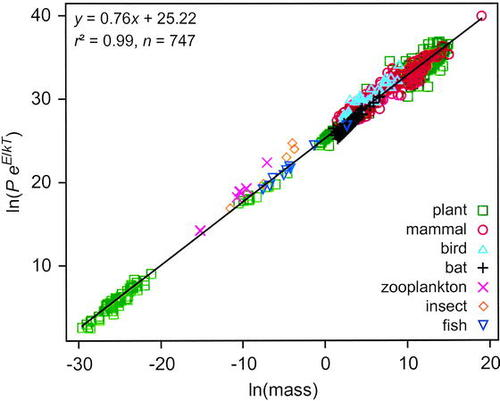
\includegraphics[width=0.8\textwidth]{../data/mass_dependence_temp.jpg}
      \caption{Mass dependence of temperature-corrected maximal rates of whole-organism biomass production.}
      \label{fig:mass_dep_temp}
      \end{center}
    \end{figure}

  \section{Discussion}

    The allometric scaling of this phenomenum applies across several orders of magnitude and levels of organization.

  \bibliographystyle{plain}
  
  \bibliography{FirstBiblio}

\end{document}